\documentclass[10pt]{beamer}

\usepackage[T1]{fontenc}

\usepackage{mathtools}
\usetheme{Montpellier}
\usepackage{tipa}
\usepackage{silence,lmodern}
\usepackage[backend=biber, style=ieee]{biblatex}
\usepackage{minted}
\hypersetup{colorlinks = true, urlcolor=blue, linkcolor=black}

\WarningFilter{biblatex}{Patching footnotes failed}

\renewcommand*{\bibfont}{\tiny}

\bibliography{resources.bib}

\title{\textbf{Operating Systems}}
\subtitle{Tutorial}
\author{Fabian Klopfer}
\date{\today}

\begin{document}

\frame{\titlepage}

\begin{frame}
  \frametitle{TOC}
  \tableofcontents[hideallsubsections]
\end{frame}
%% Check TUM Aufgaben

\begin{frame}{Intro}
\begin{itemize}
 \item Fabian, 2. Semester M.Sc. Computer \& Information Science, fabian.klopfer@uni.kn 
 \item Reminder: English Poll
 \item Fork \href{https://gitlab.inf.uni-konstanz.de/matthias.rupp/betriebssysteme/}{the repository} \& do sheet 0
 \item More organisation stuff in the lecture
 \item The following slides are preliminary as the lecture is WIP
 \item sorry for the sloppy image references!
\end{itemize}
\end{frame}

\section{Manuals \& Literature}
    \begin{frame}{Processor \& Compiler Reference}
    Not a must read for this course but a good reference for low level details: \\
        \href{https://www.amd.com/system/files/TechDocs/24593.pdf}{AMD64 Manual} \\
        \href{https://software.intel.com/content/dam/develop/public/us/en/documents/325462-sdm-vol-1-2abcd-3abcd.pdf}{Intel x86 \& x64 Manual} \\
        \href{https://uclibc.org/docs/psABI-x86\_64.pdf}{SystemV x86 Calling Convention} \\
        \href{https://www.sandpile.org/}{Comprehensive Low Level Information Collection} \\git 
    \end{frame}

    \begin{frame}{C Programming \& Operating System Reference}
        Your best friend when programming: \\
        \href{https://en.cppreference.com/w/c}{Official C Language Reference} \vspace{2cm} \\ 
        Unix \& Linux references: \\
        \href{https://linux.die.net/}{Linux Manuals (searchable!)} \\
        \href{https://linux.die.net/man/2/syscalls}{Linux Syscalls Man Page} \\
        \href{https://pubs.opengroup.org/onlinepubs/9699919799/functions/contents.html}{POSIX Specification} \\
        \href{https://tldp.org/}{The Linux Kernel Documentation Project} \\
    \end{frame}
    
    \begin{frame}{Literature hint}
    \alert{Get (digital) copies of all books!} \vspace{2cm} \\ 
    Many nice graphs: \\ 
    \href{Operating Systems: Internals and Design, William Stallings}{https://dinus.ac.id/repository/docs/ajar/Operating\_System.pdf}
    \end{frame}

\section{Operating Systems Overview}
\subsection{Overview}
\begin{frame}[allowframebreaks]{Overview}
\begin{center}
 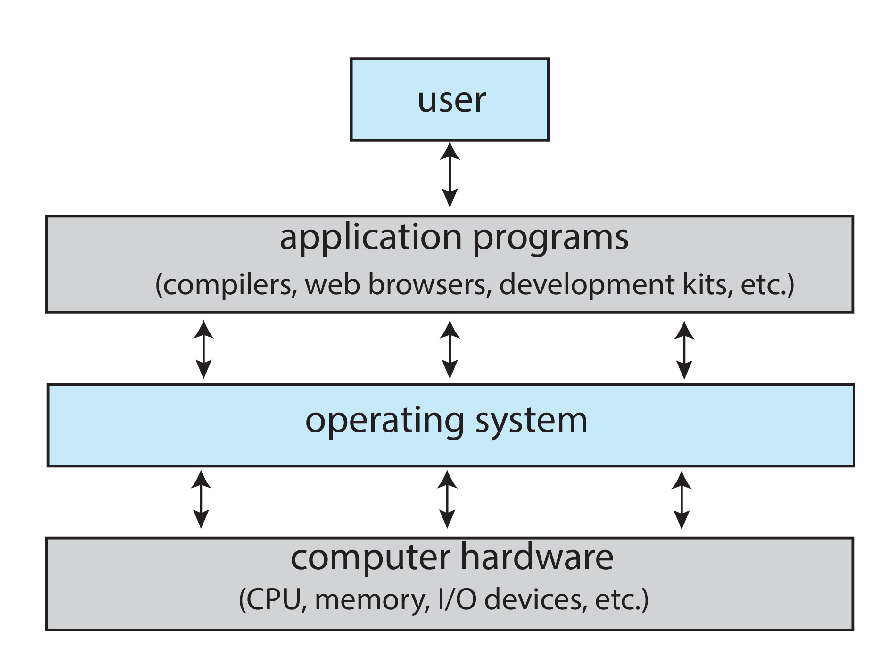
\includegraphics[keepaspectratio, width=\textwidth, height=\textheight-2\baselineskip-2\baselineskip]{img/000_software_layers.png} \\ \framebreak
  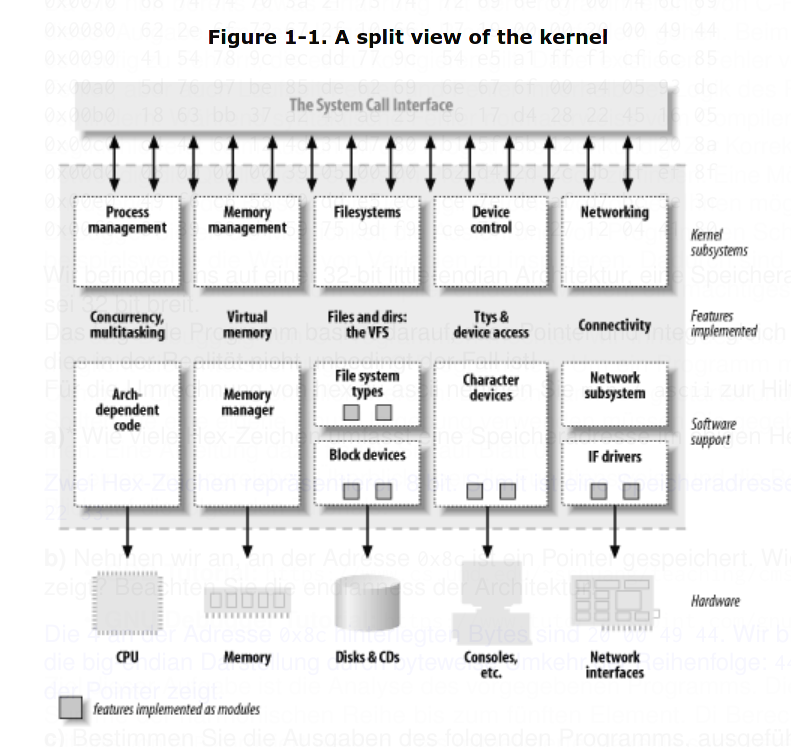
\includegraphics[keepaspectratio, width=\textwidth, height=\textheight-2\baselineskip-2\baselineskip]{img/000_kernel_split.png} \\ \framebreak
   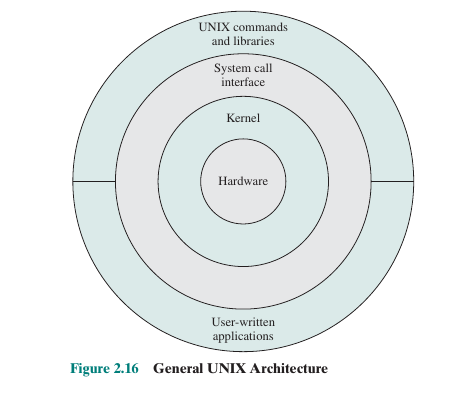
\includegraphics[keepaspectratio, width=\textwidth, height=\textheight-2\baselineskip-2\baselineskip]{img/000_rings.png} \\ \framebreak
    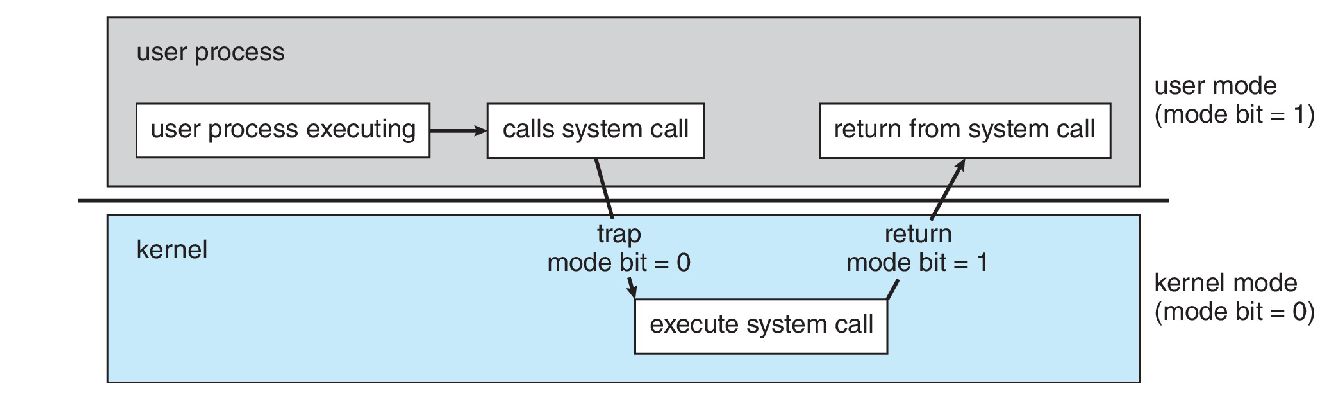
\includegraphics[keepaspectratio, width=\textwidth, height=\textheight-2\baselineskip-2\baselineskip]{img/000_mode_switch.png} \\ \framebreak
    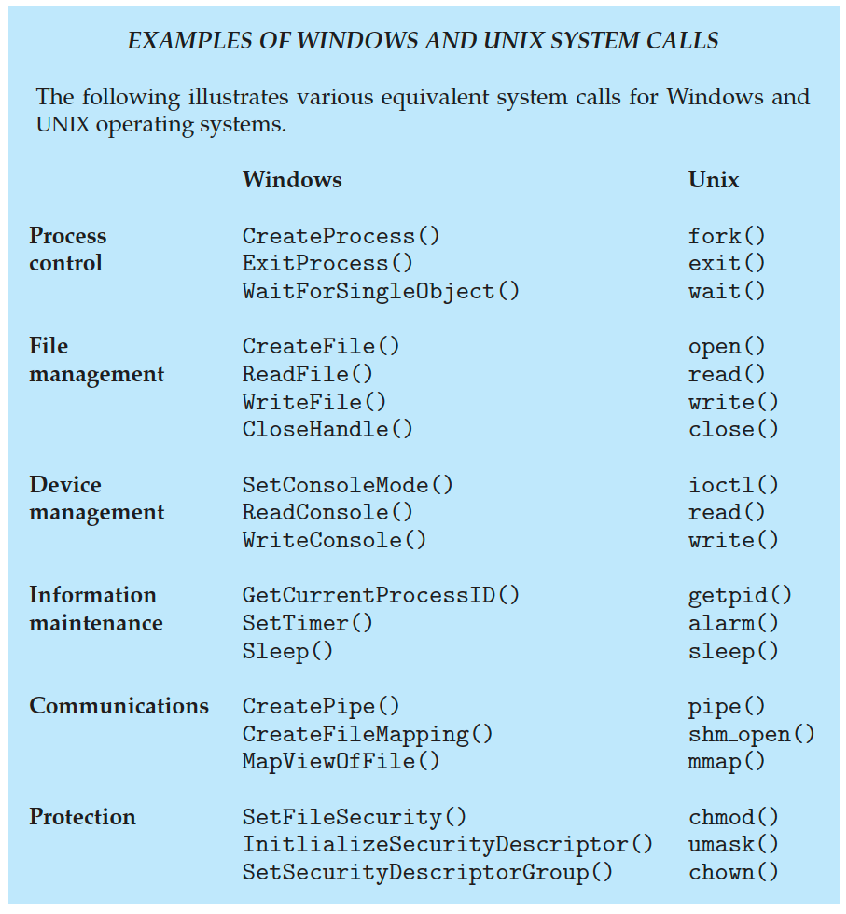
\includegraphics[keepaspectratio, width=\textwidth, height=\textheight-2\baselineskip-2\baselineskip]{img/000_sys_calls.png} \\
\end{center}
\end{frame}

\begin{frame}[allowframebreaks]{Hardware}
\begin{center}
    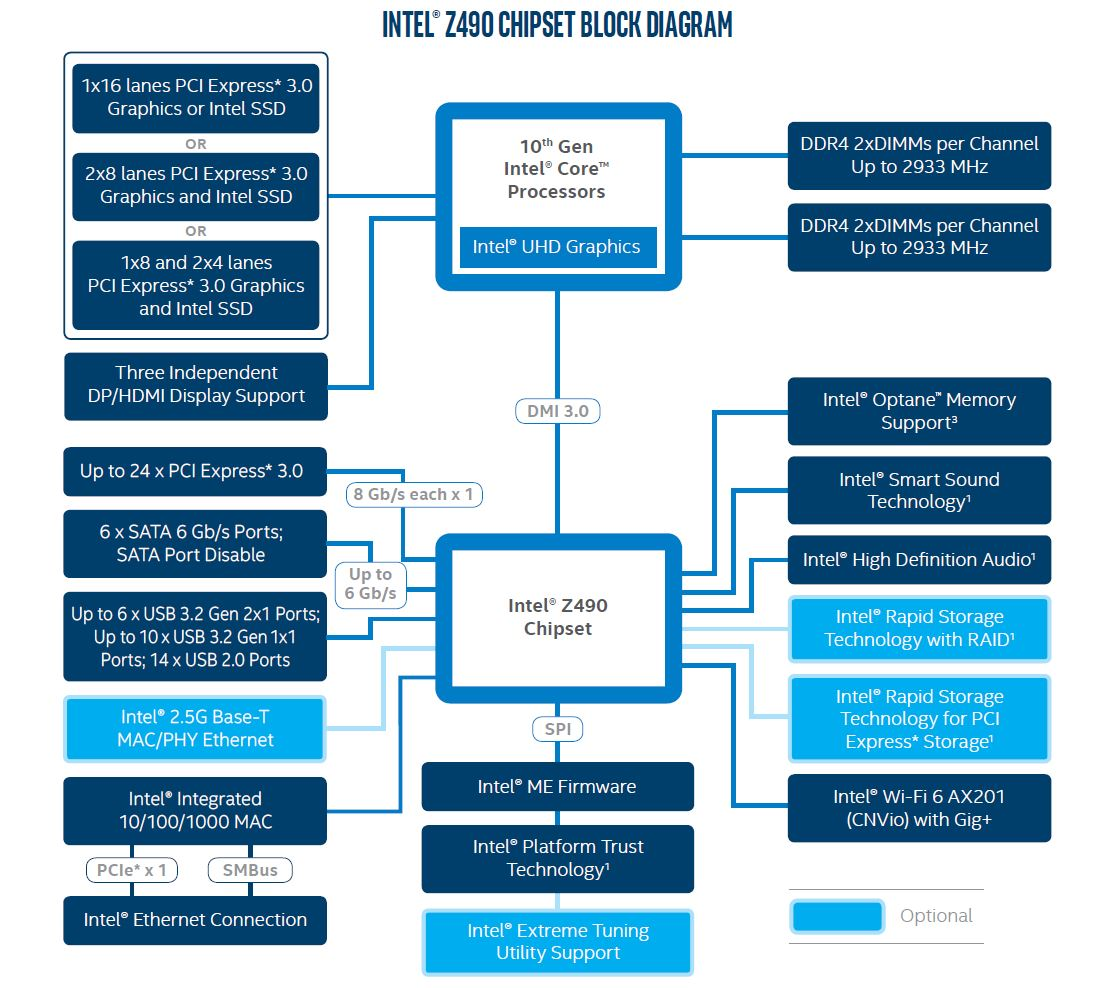
\includegraphics[keepaspectratio, width=\textwidth, height=\textheight-2\baselineskip-2\baselineskip]{img/001_chipset.jpg} \\ \framebreak
    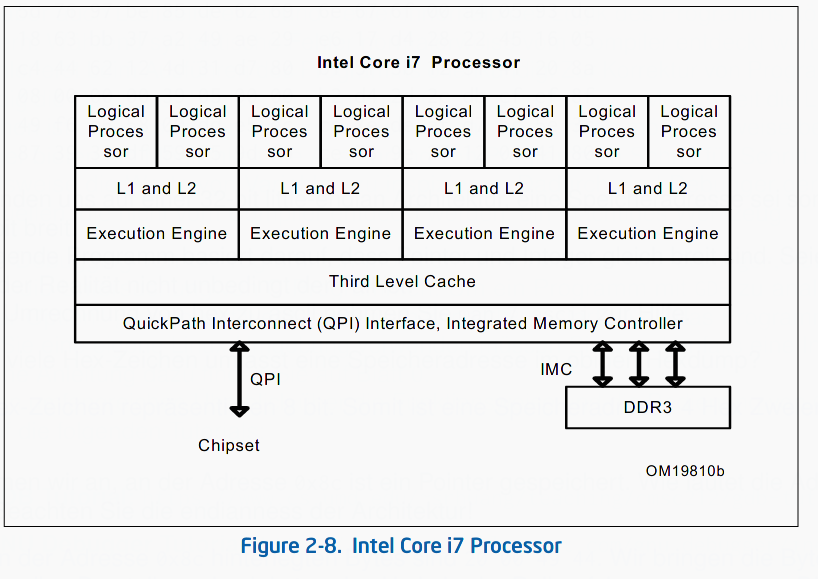
\includegraphics[keepaspectratio, width=\textwidth, height=\textheight-2\baselineskip-2\baselineskip]{img/001_i7.png} \\ \framebreak
    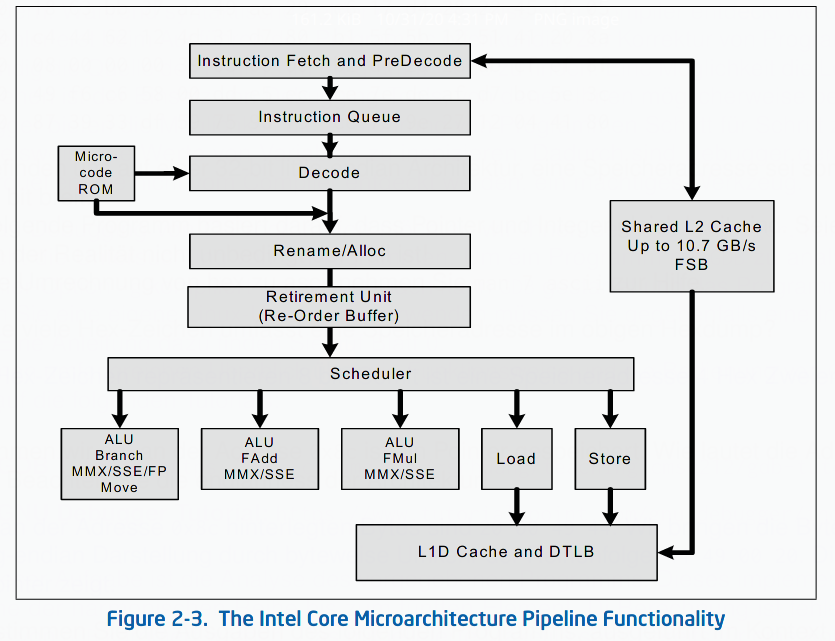
\includegraphics[keepaspectratio, width=\textwidth, height=\textheight-2\baselineskip-2\baselineskip]{img/001_execution_engine_i7.png} \\ \framebreak
    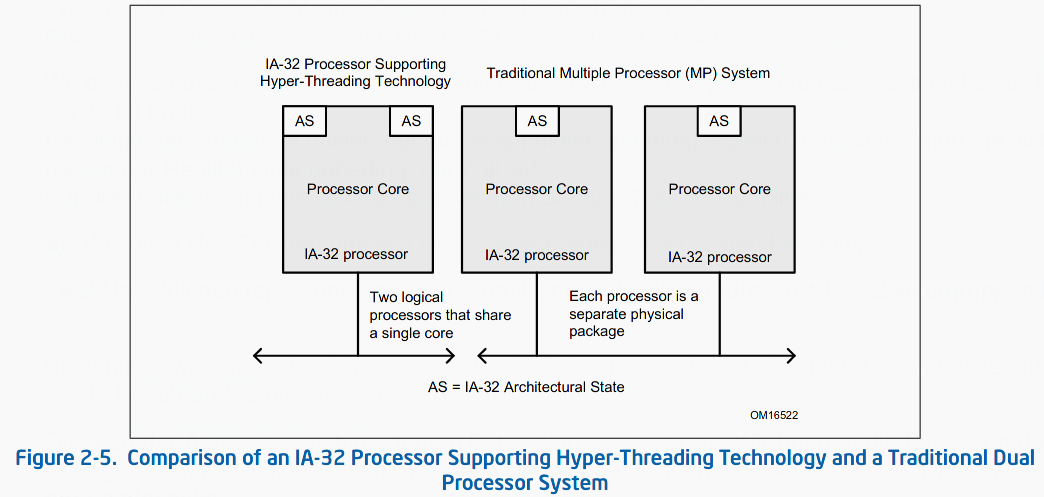
\includegraphics[keepaspectratio, width=\textwidth, height=\textheight-2\baselineskip-2\baselineskip]{img/001_hyperthreadding.png} \\ \framebreak
    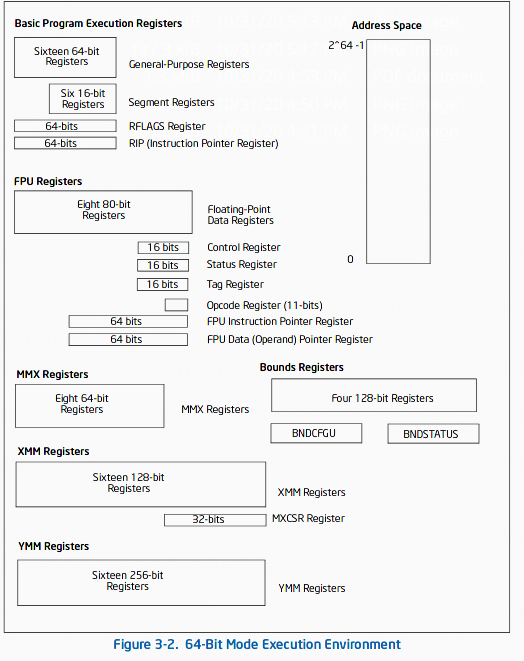
\includegraphics[keepaspectratio, width=\textwidth, height=\textheight-2\baselineskip-2\baselineskip]{img/001_registers.png} \\ \framebreak
    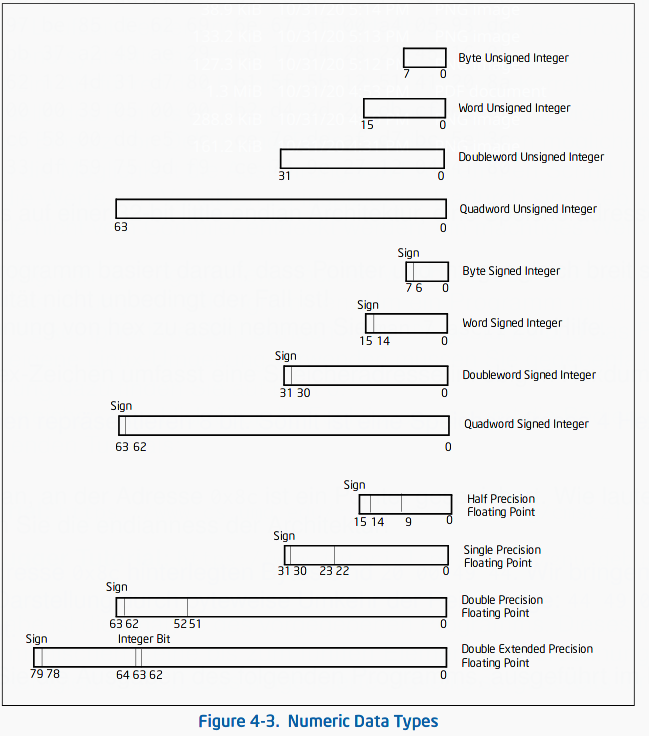
\includegraphics[keepaspectratio, width=\textwidth, height=\textheight-2\baselineskip-2\baselineskip]{img/001_data_types.png} \\
    \end{center}
\end{frame}

\subsection{Virtualization}
\begin{frame}[allowframebreaks]{Processes \& Thread}
 \begin{center}
    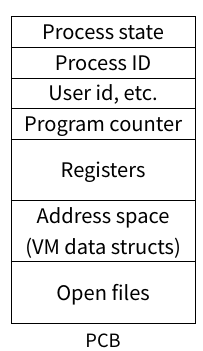
\includegraphics[keepaspectratio, width=\textwidth, height=\textheight-2\baselineskip-2\baselineskip]{img/010_pcb.png} \\ \framebreak
    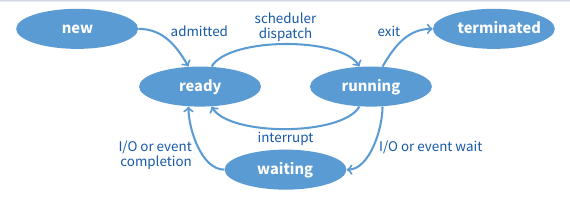
\includegraphics[keepaspectratio, width=\textwidth, height=\textheight-2\baselineskip-2\baselineskip]{img/010_proc_state.png} \\ \framebreak
    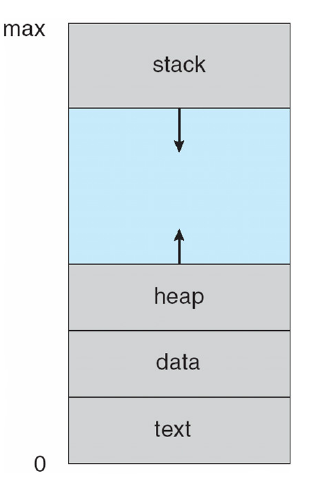
\includegraphics[keepaspectratio, width=\textwidth, height=\textheight-2\baselineskip-2\baselineskip]{img/010_process_memory.png} \\ \framebreak
    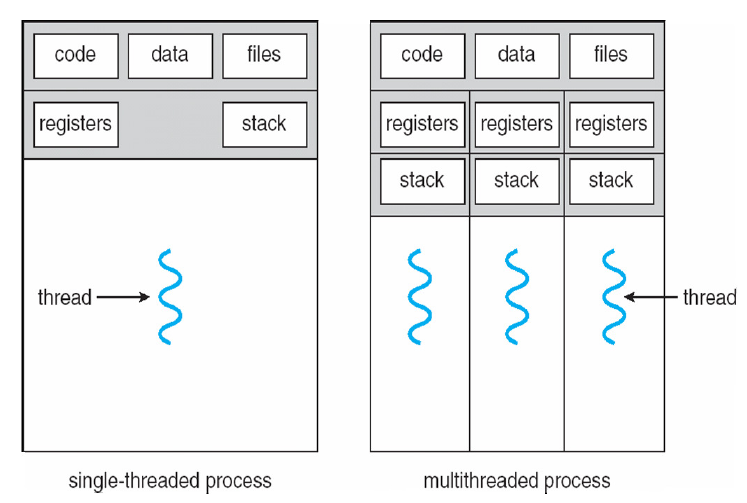
\includegraphics[keepaspectratio, width=\textwidth, height=\textheight-2\baselineskip-2\baselineskip]{img/010_proc_threads.png} \\ \framebreak
    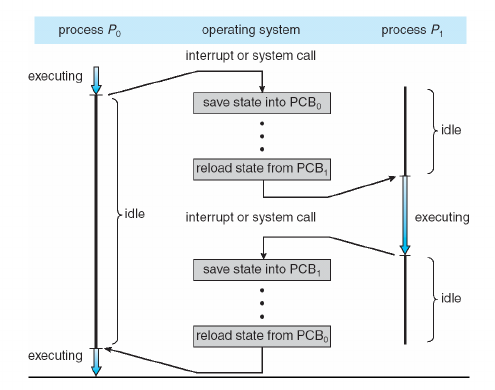
\includegraphics[keepaspectratio, width=\textwidth, height=\textheight-2\baselineskip-2\baselineskip]{img/010_context_switch.png} \\
  \end{center}
\end{frame}

\begin{frame}[allowframebreaks]{Scheduling}
 \begin{center}
    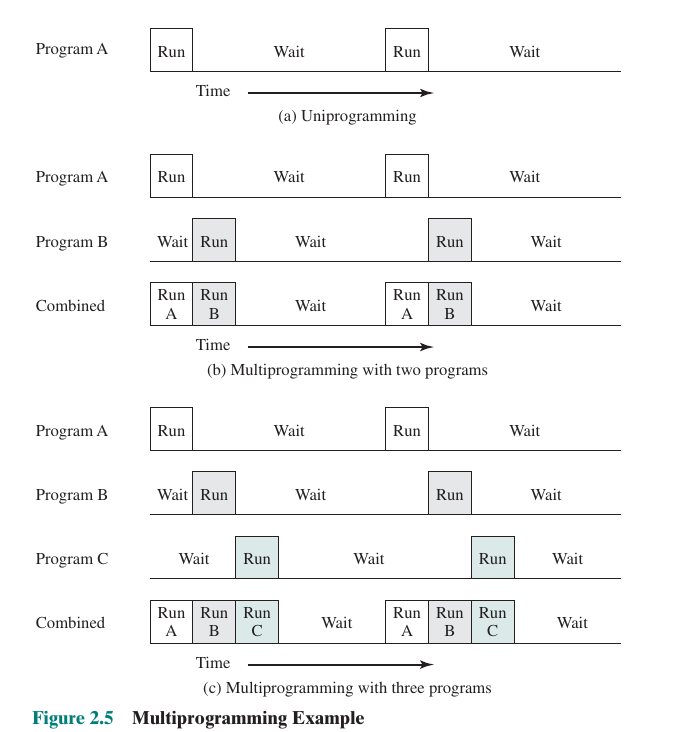
\includegraphics[keepaspectratio, width=\textwidth, height=\textheight-2\baselineskip-2\baselineskip]{img/011_sched__.png} \\ \framebreak
    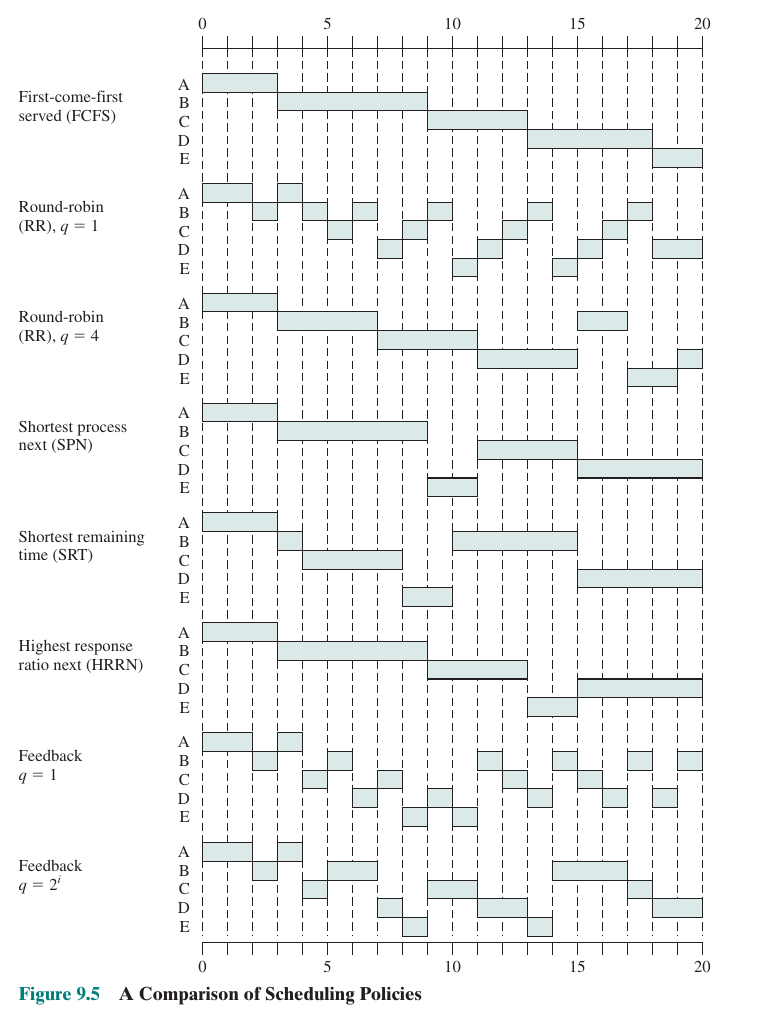
\includegraphics[keepaspectratio, width=\textwidth, height=\textheight-2\baselineskip-2\baselineskip]{img/011_sched___.png} \\ \framebreak
    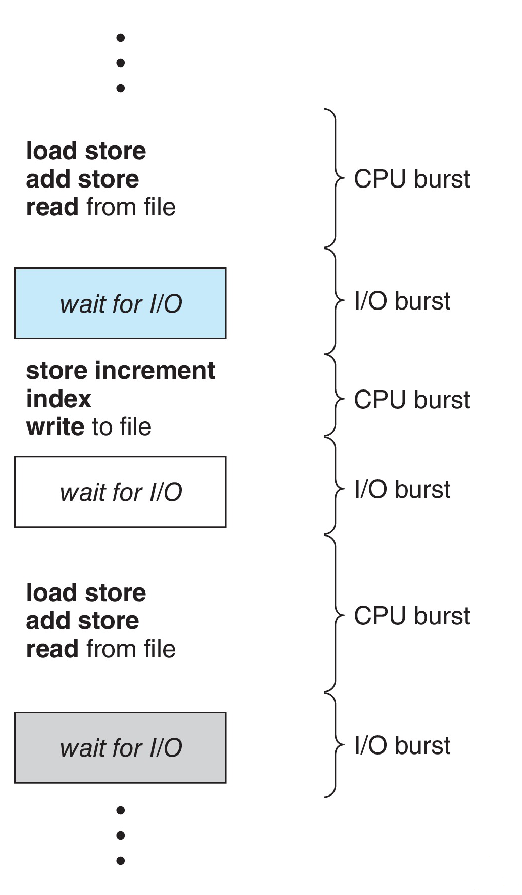
\includegraphics[keepaspectratio, width=\textwidth, height=\textheight-2\baselineskip-2\baselineskip]{img/011_bursts.png} \\ \framebreak
    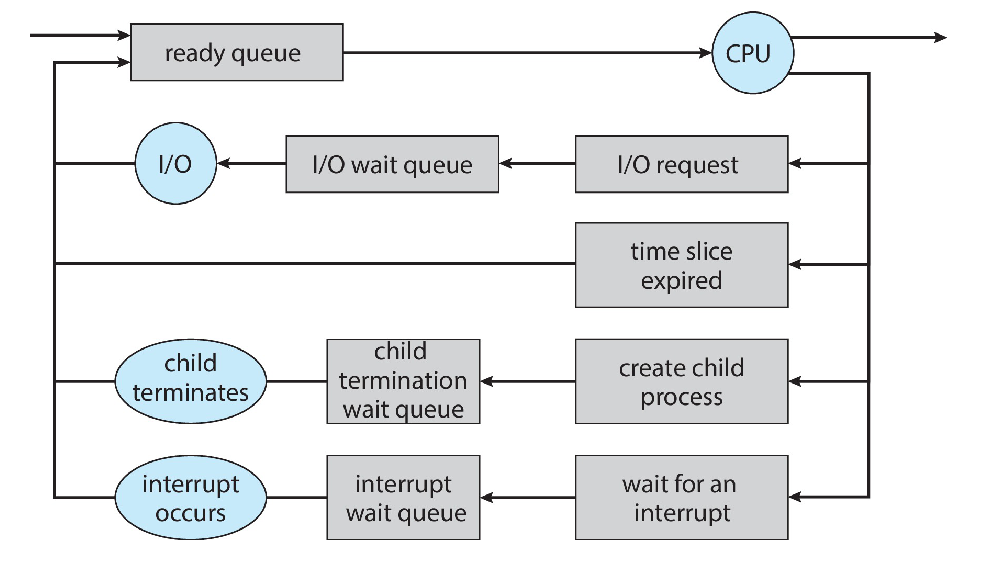
\includegraphics[keepaspectratio, width=\textwidth, height=\textheight-2\baselineskip-2\baselineskip]{img/011_sched.png} \\ \framebreak
    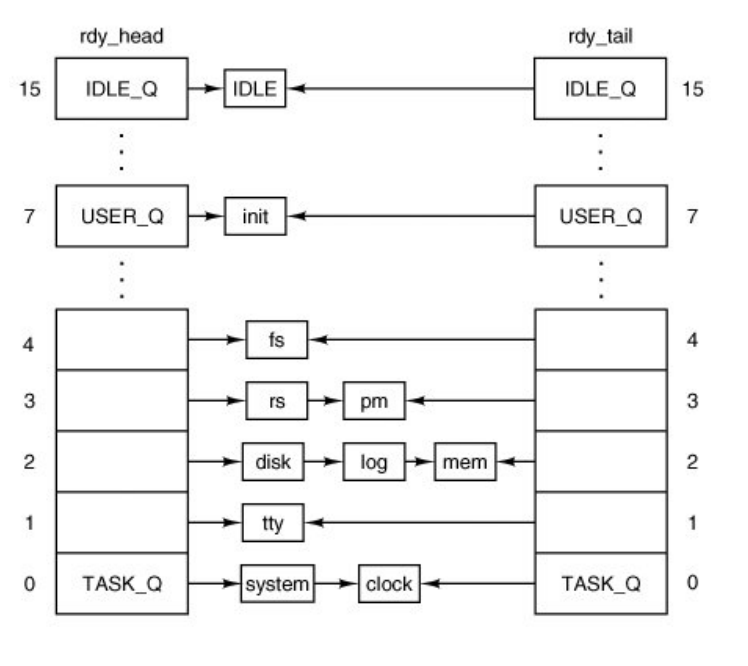
\includegraphics[keepaspectratio, width=\textwidth, height=\textheight-2\baselineskip-2\baselineskip]{img/011_sched_.png} \\
 \end{center}
\end{frame}

\begin{frame}[allowframebreaks]{Memory Management}
  \begin{center}
  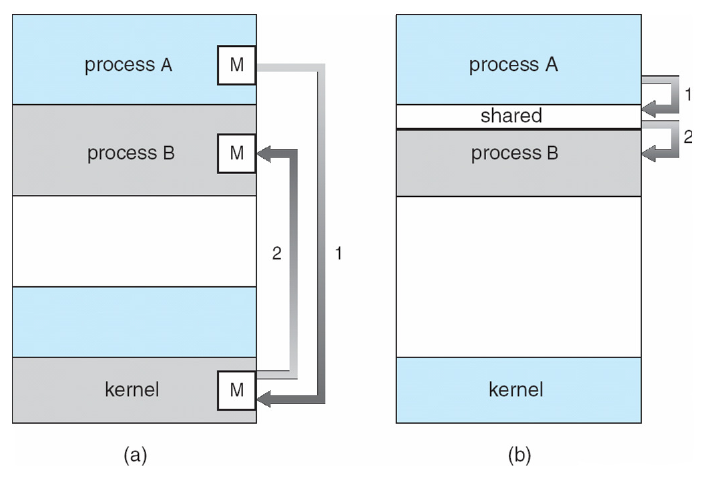
\includegraphics[keepaspectratio, width=\textwidth, height=\textheight-2\baselineskip-2\baselineskip]{img/012_mem_map.png} \\ \framebreak
    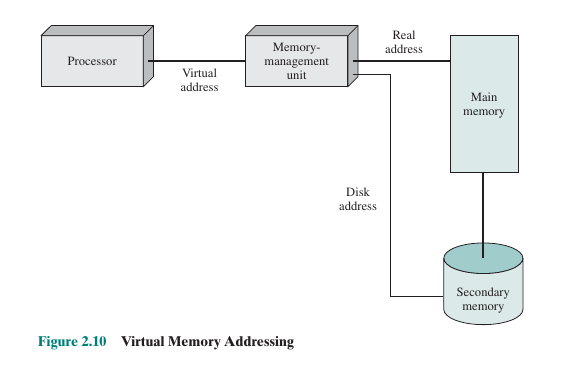
\includegraphics[keepaspectratio, width=\textwidth, height=\textheight-2\baselineskip-2\baselineskip]{img/012_mmu.png} \\ \framebreak
    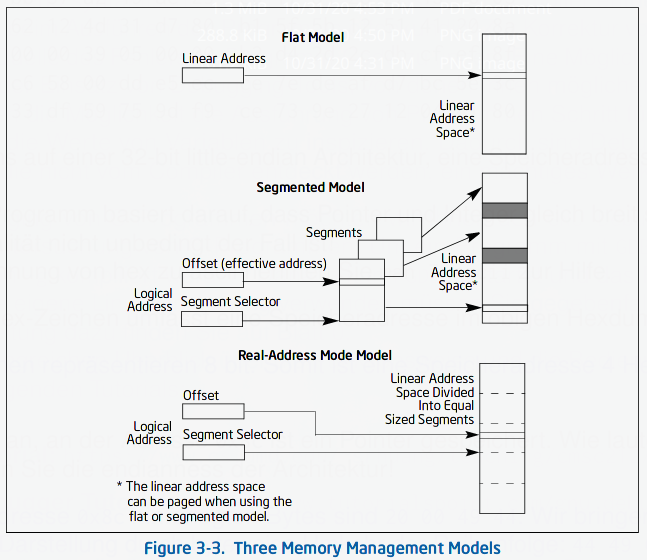
\includegraphics[keepaspectratio, width=\textwidth, height=\textheight-2\baselineskip-2\baselineskip]{img/012_mem_model.png} \\ \framebreak
    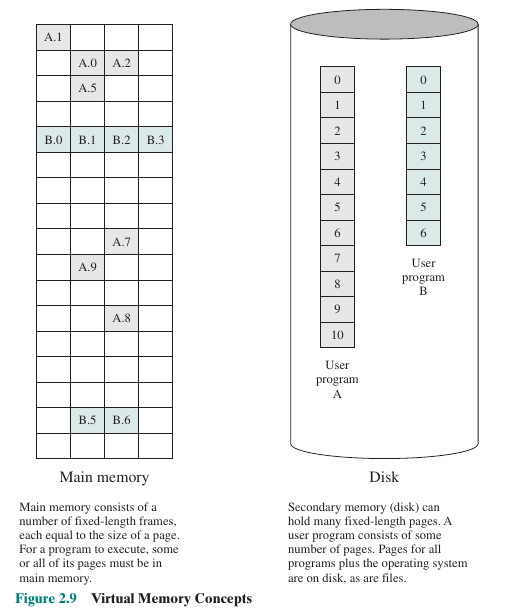
\includegraphics[keepaspectratio, width=\textwidth, height=\textheight-2\baselineskip-2\baselineskip]{img/012_paging.png} \\ \framebreak
    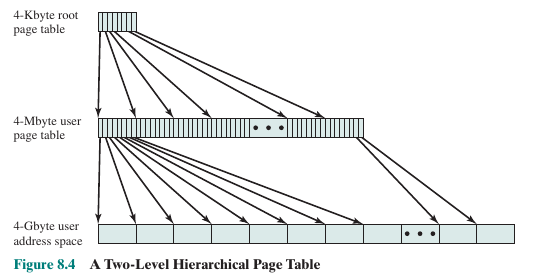
\includegraphics[keepaspectratio, width=\textwidth, height=\textheight-2\baselineskip-2\baselineskip]{img/012_page_table.png} \\ \framebreak
    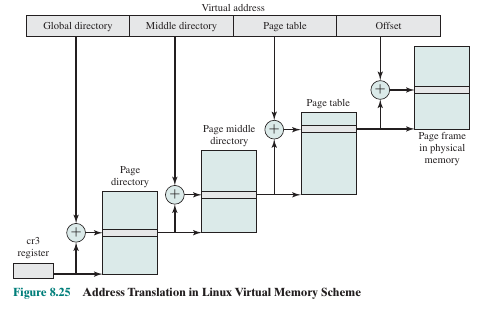
\includegraphics[keepaspectratio, width=\textwidth, height=\textheight-2\baselineskip-2\baselineskip]{img/012_paging_linux.png} \\ \framebreak
    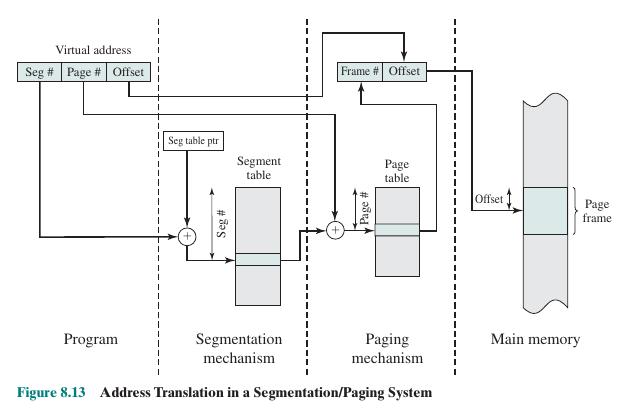
\includegraphics[keepaspectratio, width=\textwidth, height=\textheight-2\baselineskip-2\baselineskip]{img/012_paging_seg.png} \\
 \end{center}
\end{frame}

\begin{frame}{Virtual Systems}
 \begin{center}
      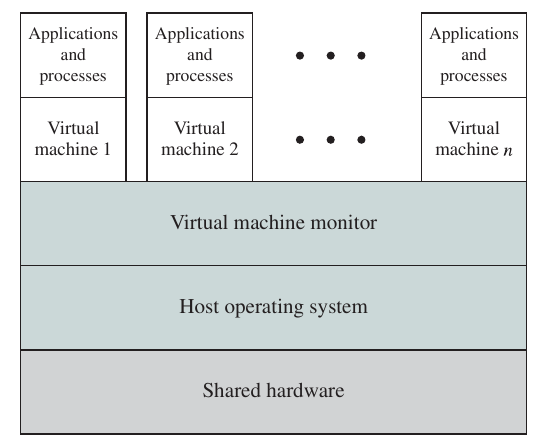
\includegraphics[keepaspectratio, width=\textwidth, height=\textheight-2\baselineskip-2\baselineskip]{img/013_virtual_machine.png} \\ 
 \end{center}
\end{frame}

\subsection{Concurrency}
\begin{frame}[allowframebreaks]{Concurrency \& Parallelism}
  \begin{center}
      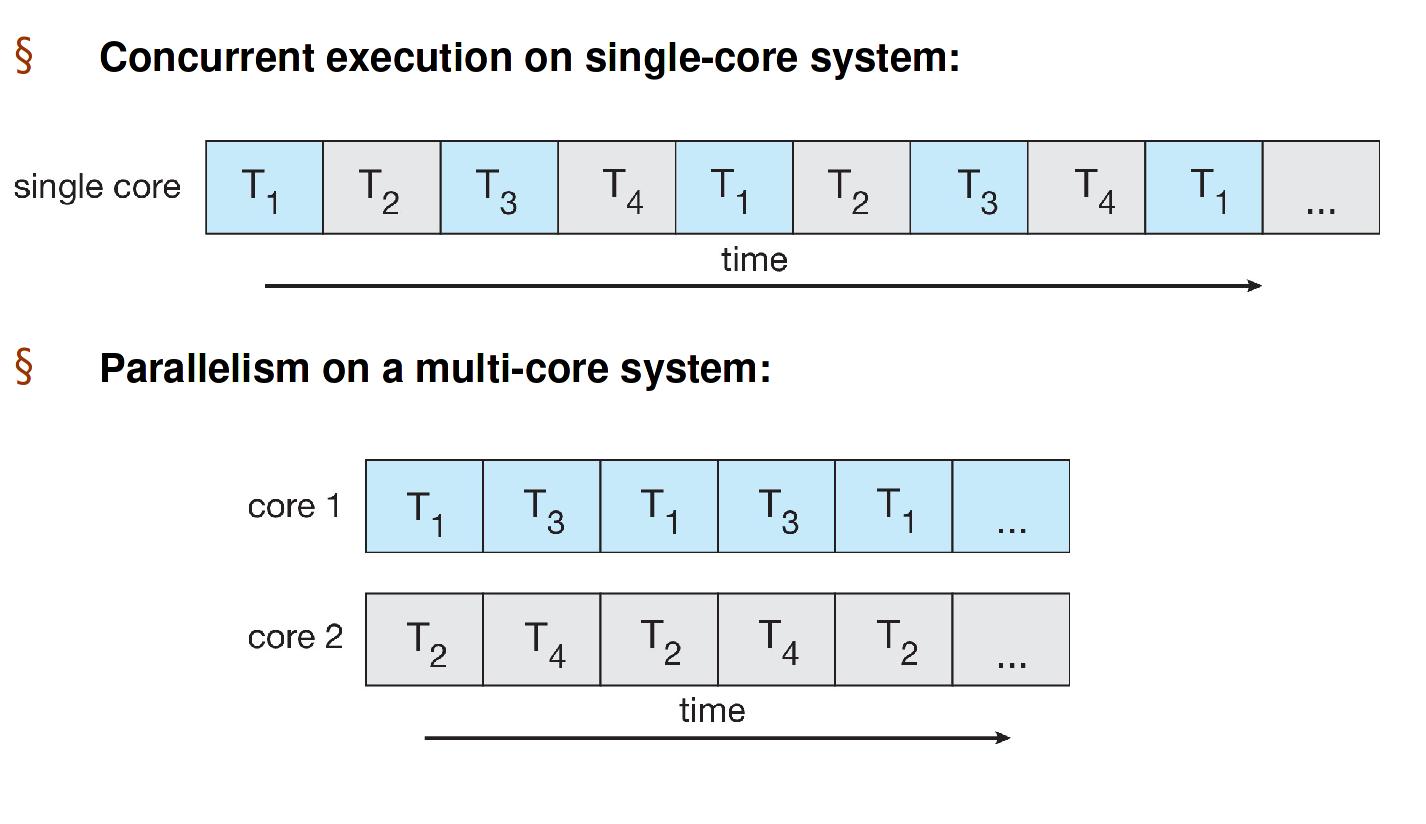
\includegraphics[keepaspectratio, width=\textwidth, height=\textheight-2\baselineskip-2\baselineskip]{img/020_concurrency_parallelism.png} \\ \framebreak
      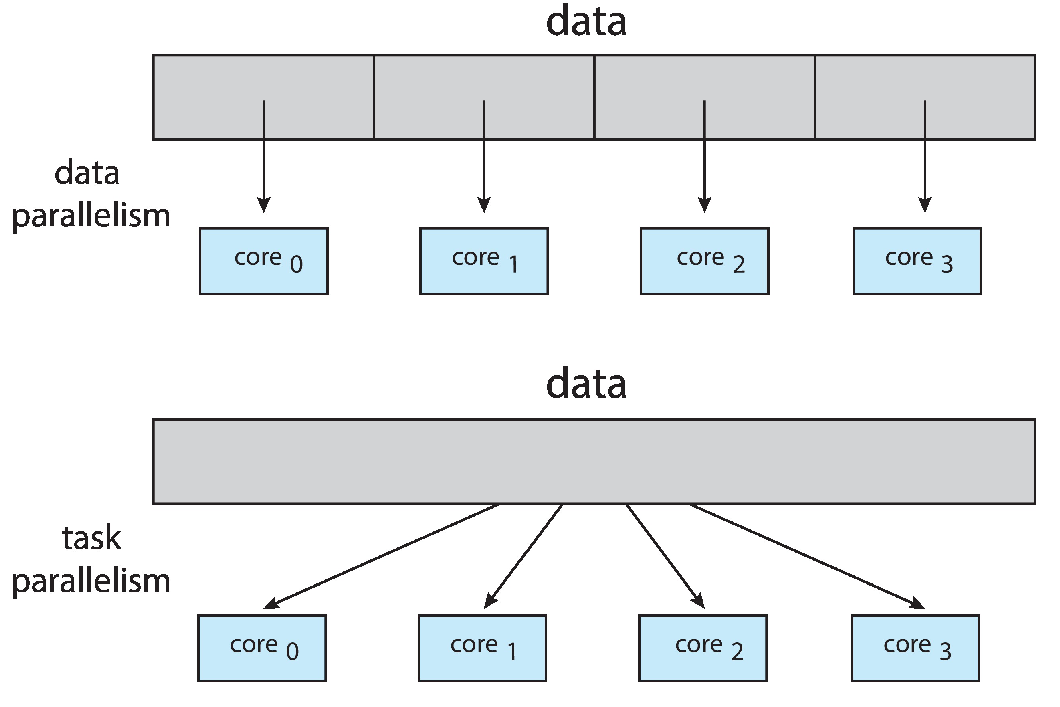
\includegraphics[keepaspectratio, width=\textwidth, height=\textheight-2\baselineskip-2\baselineskip]{img/020_parallelism_data_task.png} \\
 \end{center}
\end{frame}

\begin{frame}{Race Condition}
   \begin{center}
      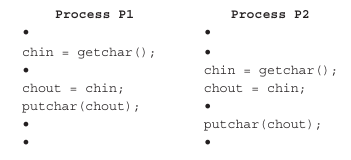
\includegraphics[keepaspectratio, width=\textwidth, height=\textheight-2\baselineskip-2\baselineskip]{img/021_race_cond.png} \\
 \end{center}
\end{frame}

\begin{frame}{Synchronization}
    \begin{center}
      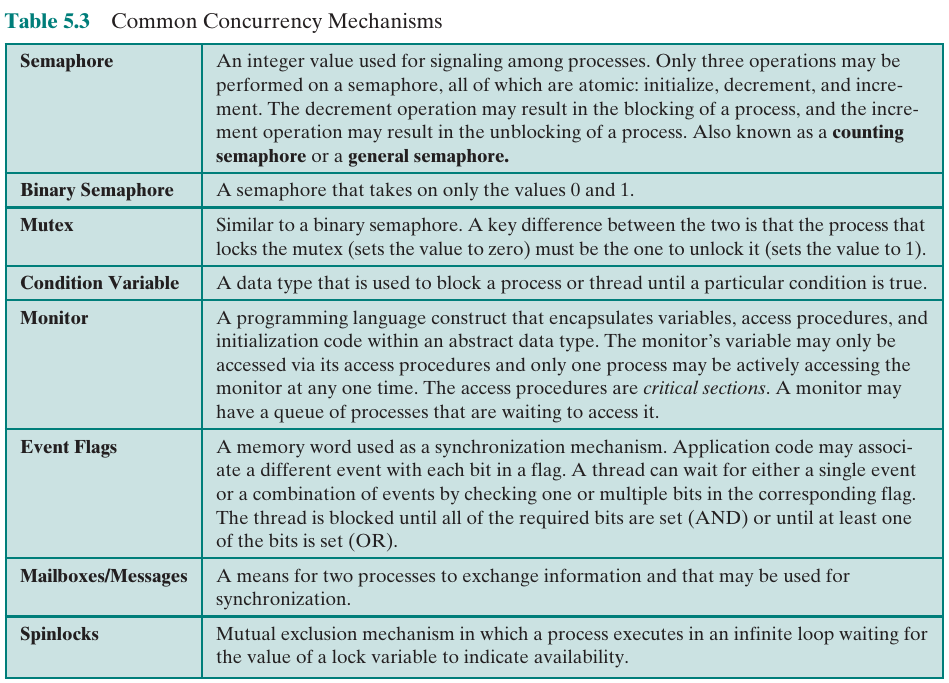
\includegraphics[keepaspectratio, width=\textwidth, height=\textheight-2\baselineskip-2\baselineskip]{img/022_locks.png} \\
 \end{center}
\end{frame}

\begin{frame}[allowframebreaks]{Deadlocks}
  \begin{center}
      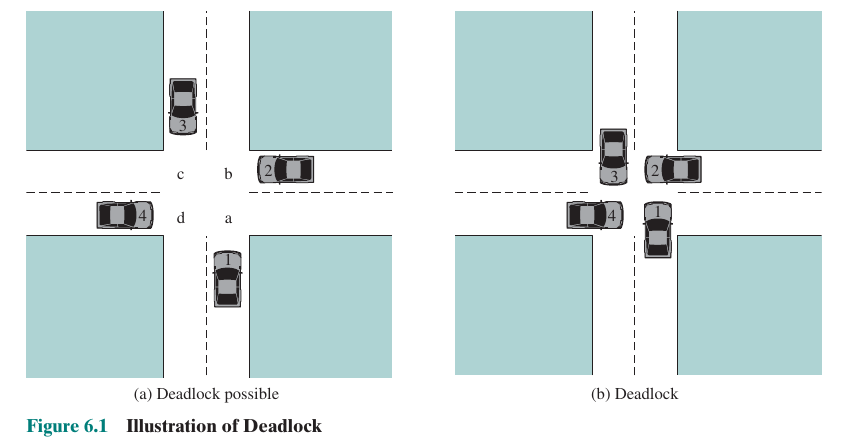
\includegraphics[keepaspectratio, width=\textwidth, height=\textheight-2\baselineskip-2\baselineskip]{img/023_deadlock.png} \\ \framebreak
      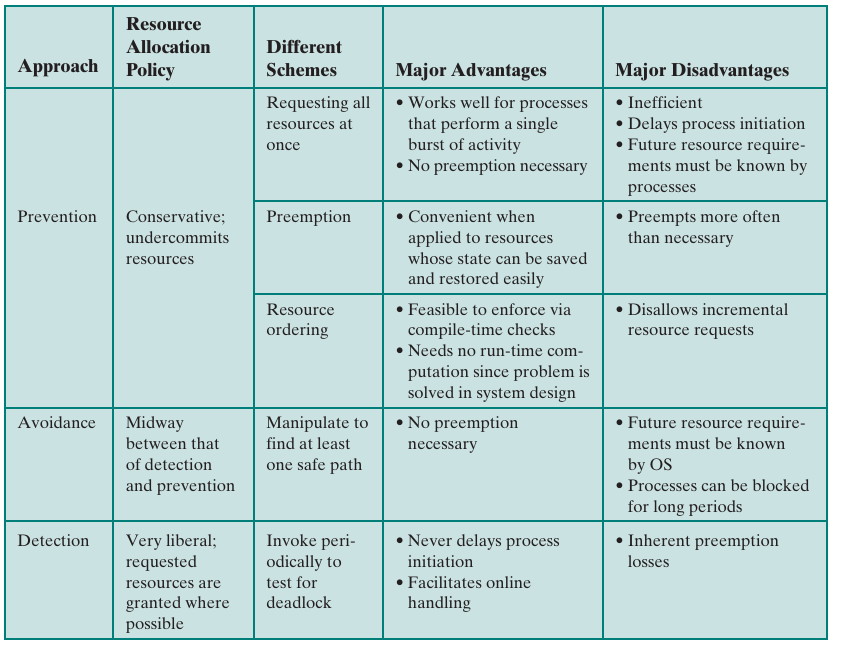
\includegraphics[keepaspectratio, width=\textwidth, height=\textheight-2\baselineskip-2\baselineskip]{img/023_deadlock_fix.png} \\
 \end{center}
\end{frame}

\subsection{I/O}
\begin{frame}[allowframebreaks]{Devices \& Drivers}
   \begin{center}
      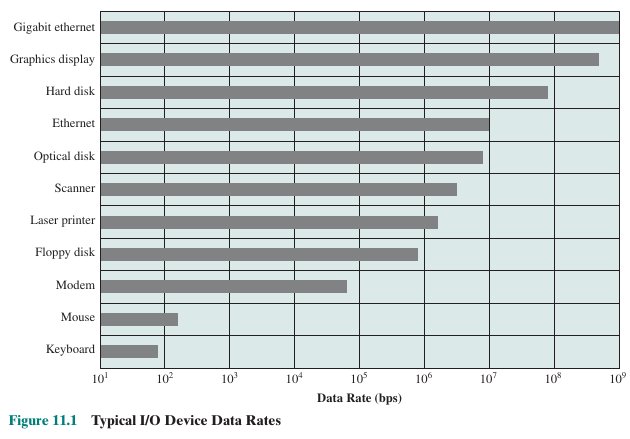
\includegraphics[keepaspectratio, width=\textwidth, height=\textheight-2\baselineskip-2\baselineskip]{img/030_io_rates.png} \\ \framebreak
      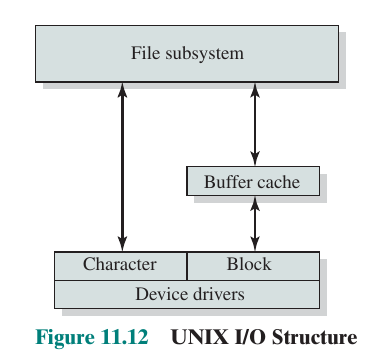
\includegraphics[keepaspectratio, width=\textwidth, height=\textheight-2\baselineskip-2\baselineskip]{img/030_io_types.png} \\ \framebreak
      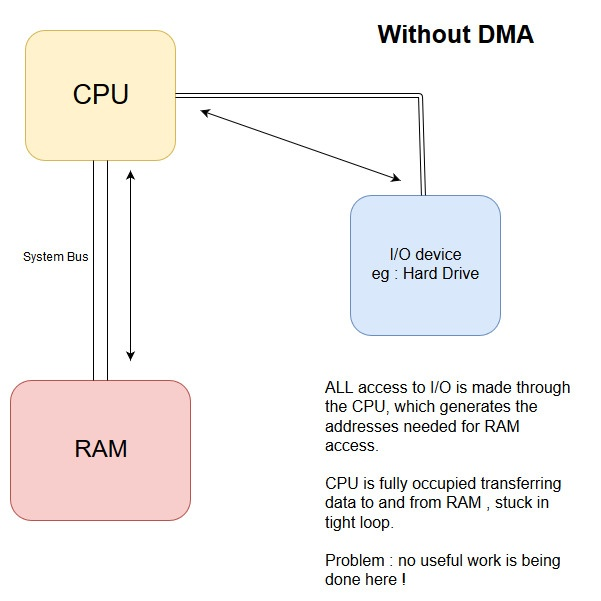
\includegraphics[keepaspectratio, width=\textwidth, height=\textheight-2\baselineskip-2\baselineskip]{img/030_no_dma.jpg} \\ \framebreak
      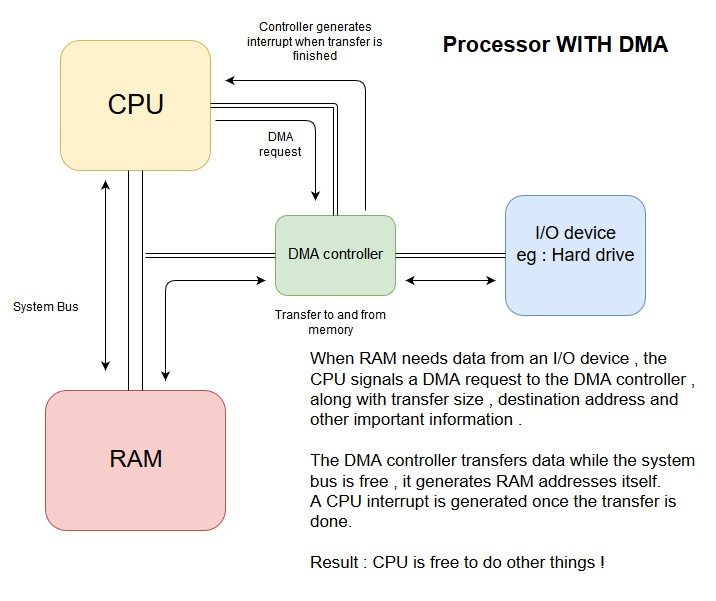
\includegraphics[keepaspectratio, width=\textwidth, height=\textheight-2\baselineskip-2\baselineskip]{img/030_dma.jpg} \\ \framebreak
      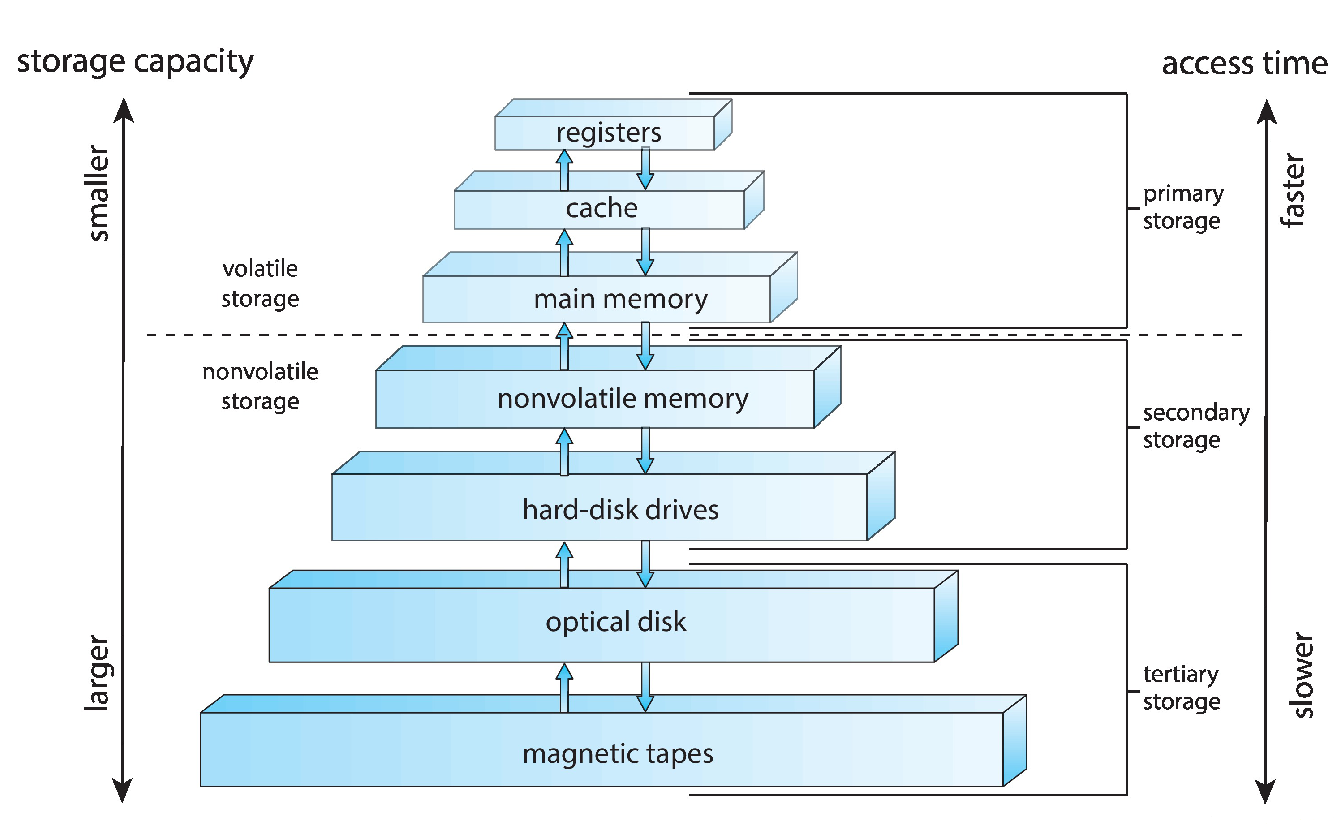
\includegraphics[keepaspectratio, width=\textwidth, height=\textheight-2\baselineskip-2\baselineskip]{img/030_storage_hierarchy.png} \\ \framebreak
      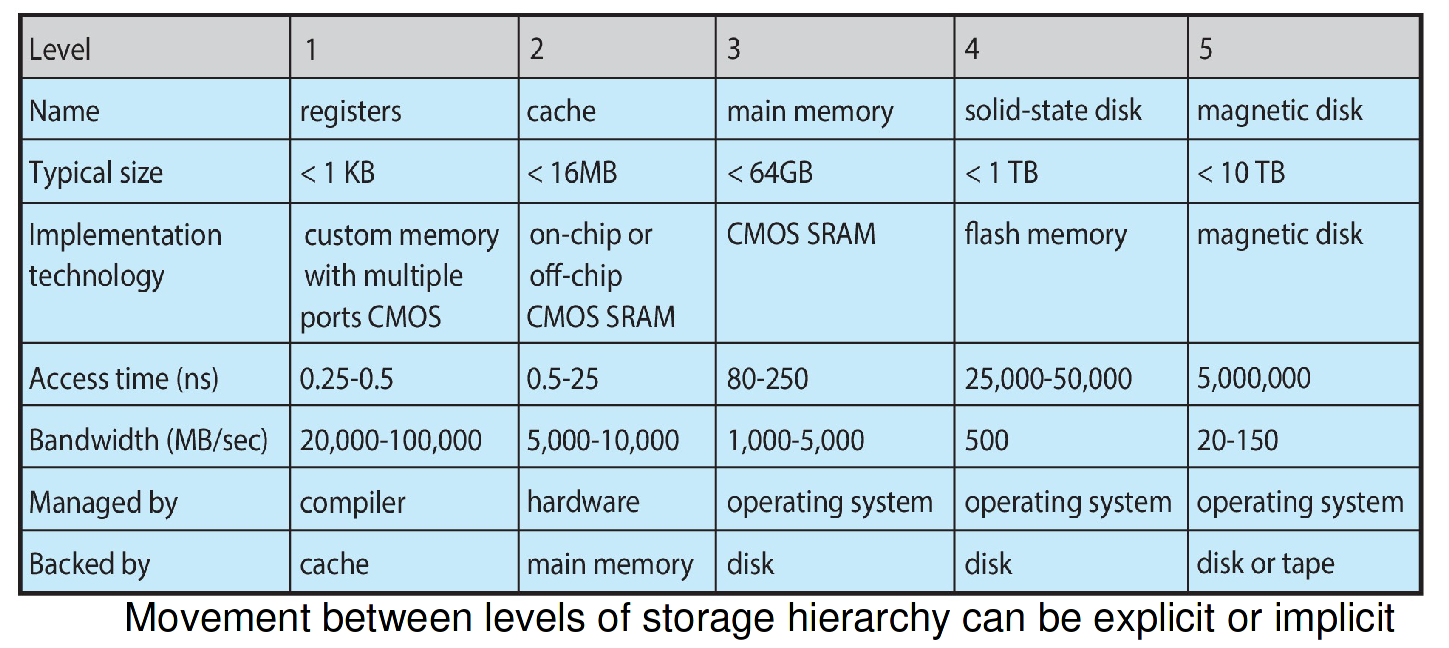
\includegraphics[keepaspectratio, width=\textwidth, height=\textheight-2\baselineskip-2\baselineskip]{img/030_storage_details.png} \\
 \end{center}
\end{frame}

\begin{frame}[allowframebreaks]{File Systems}
   \begin{center}
      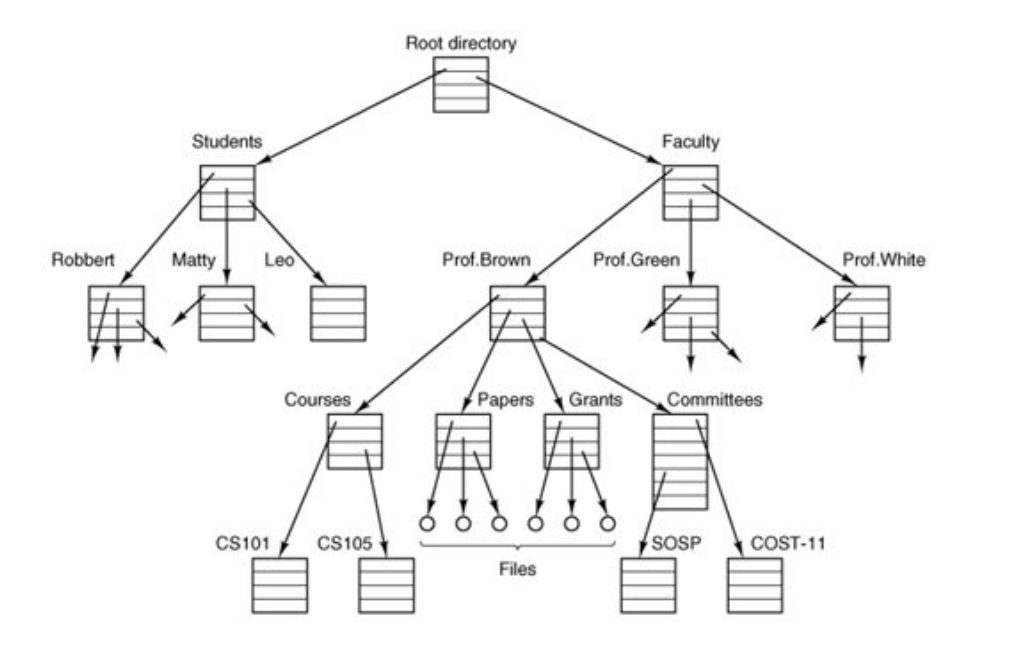
\includegraphics[keepaspectratio, width=\textwidth, height=\textheight-2\baselineskip-2\baselineskip]{img/031_filesys.png} \\ \framebreak
      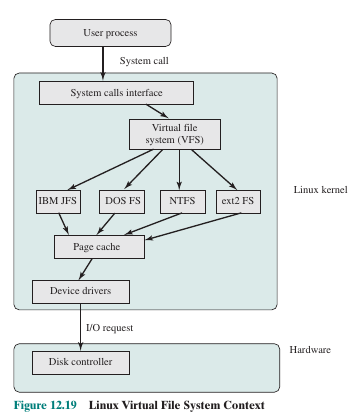
\includegraphics[keepaspectratio, width=\textwidth, height=\textheight-2\baselineskip-2\baselineskip]{img/031_fs_linux.png} \\
 \end{center}
\end{frame}


\begin{frame}{All in One Map}
Take 5 min to explore the \href{https://makelinux.github.io/kernel/map/}{map}!
 \begin{center}
      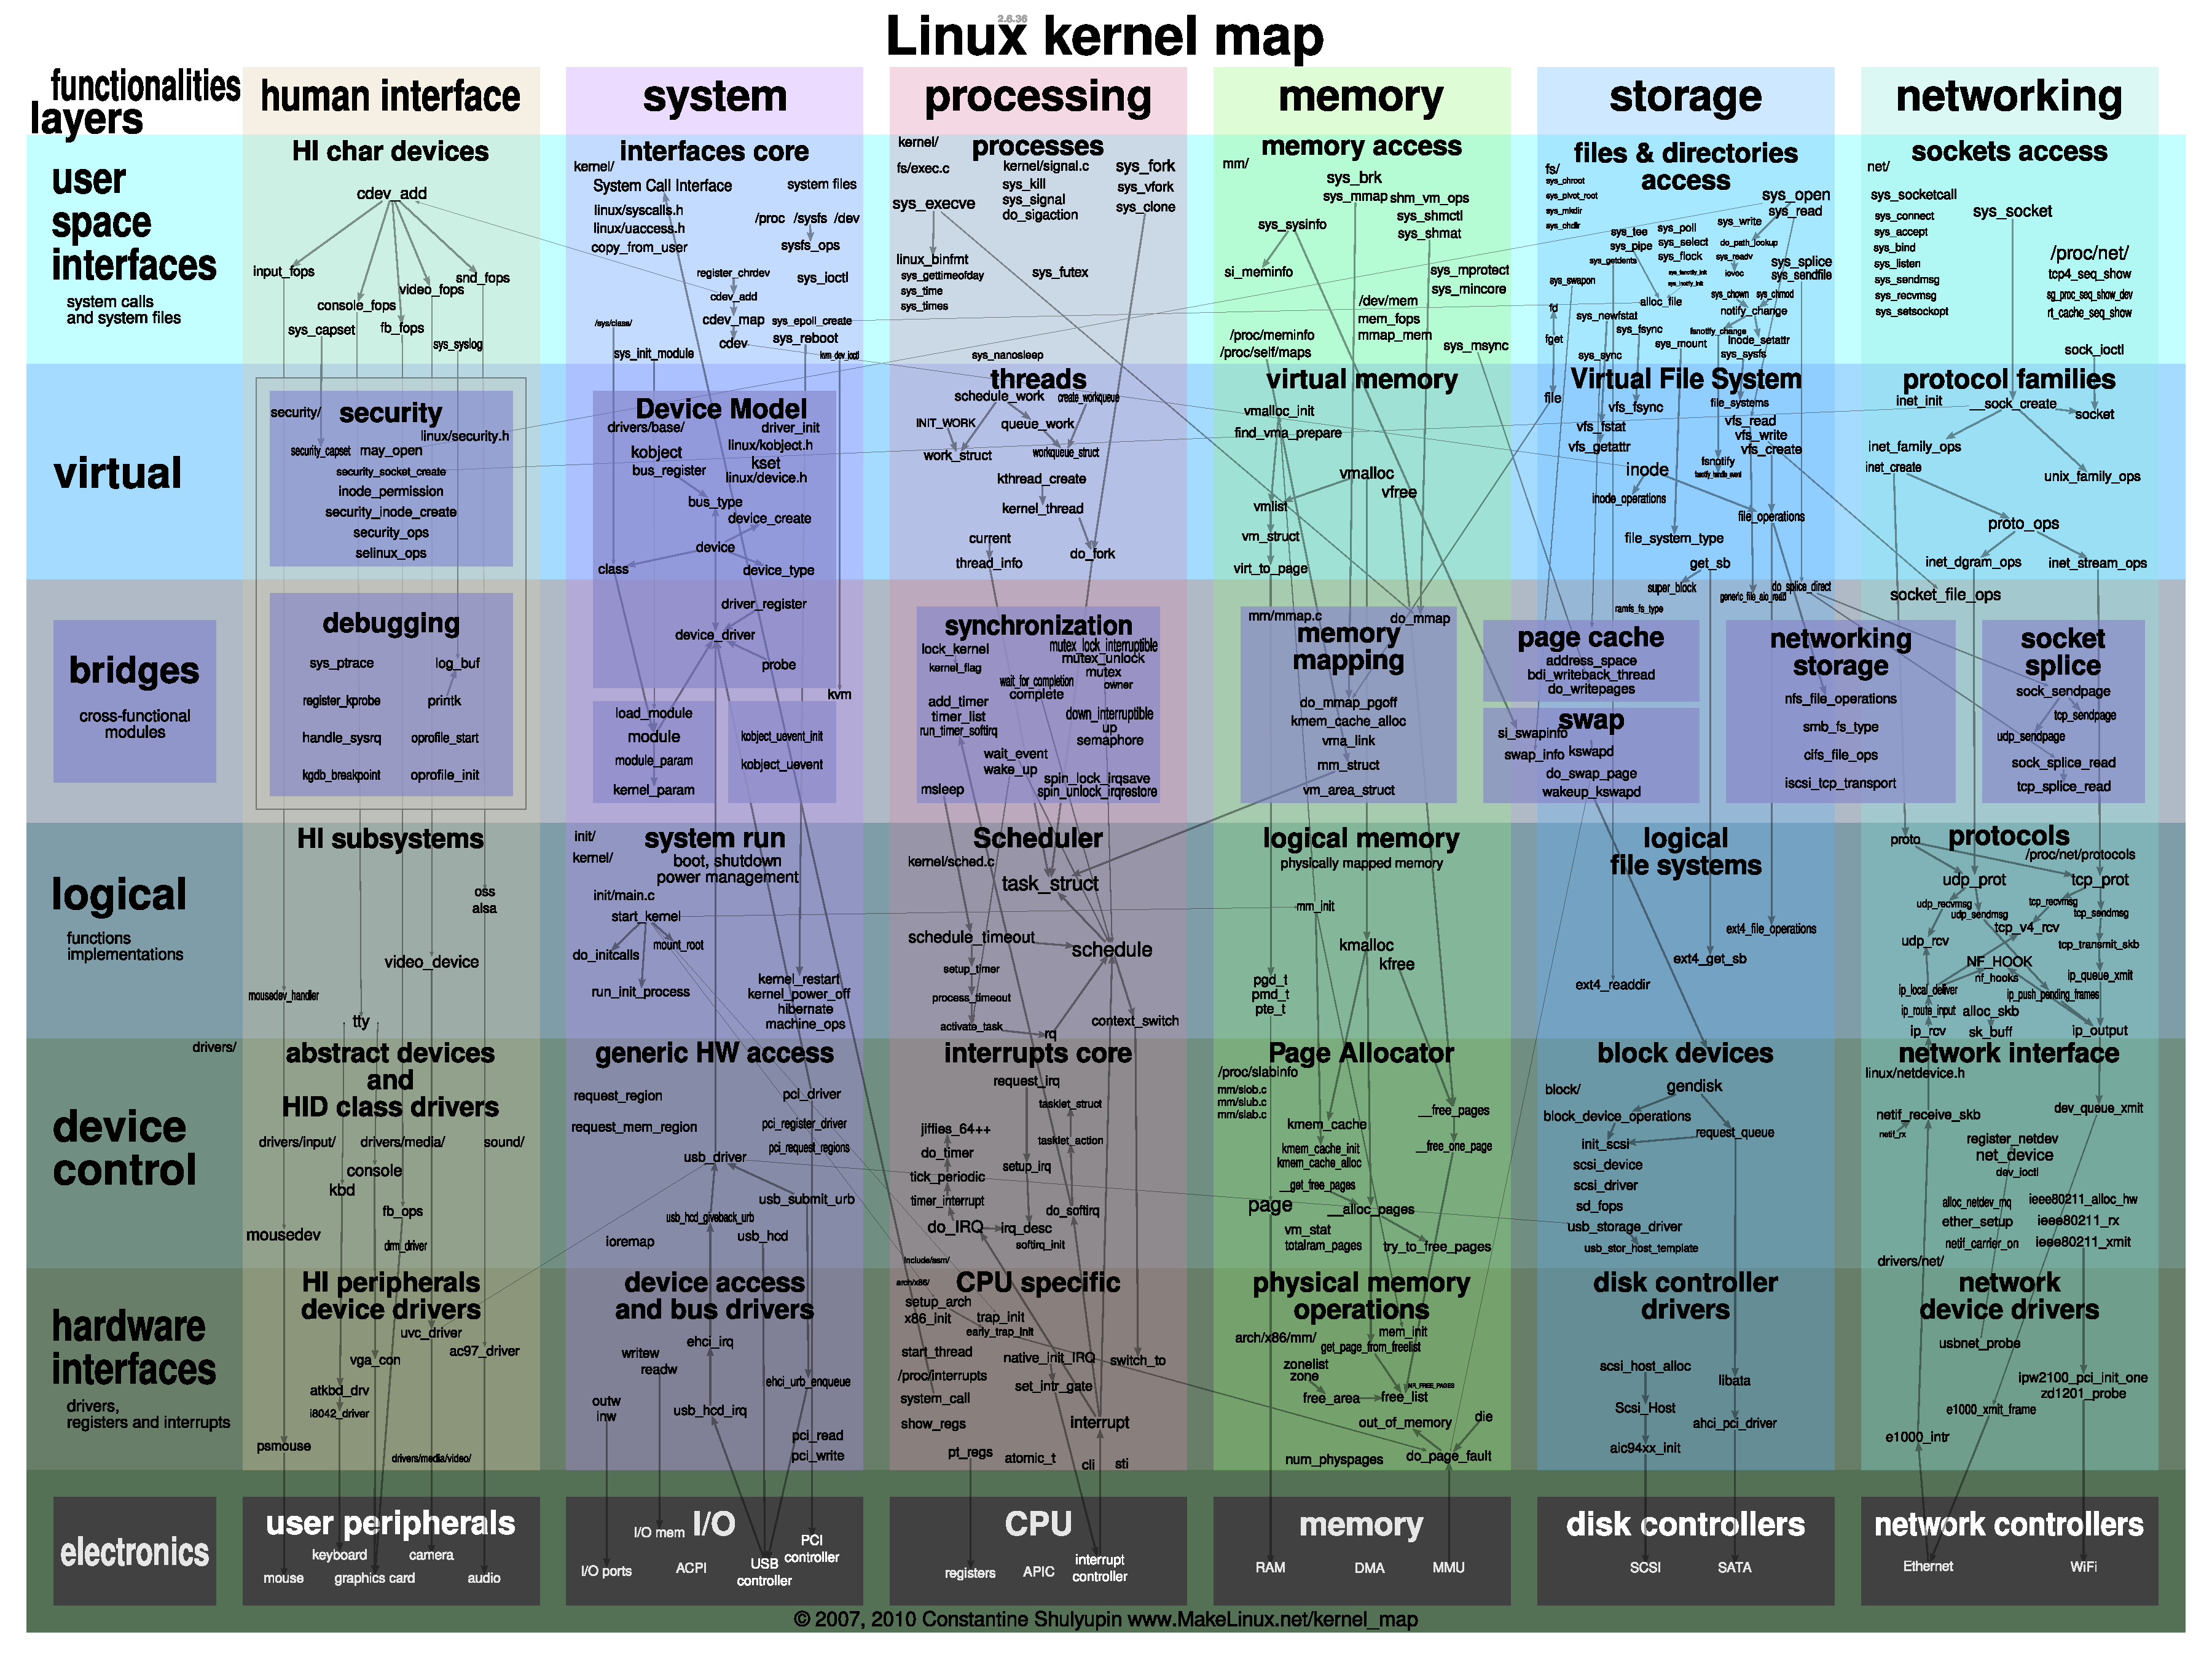
\includegraphics[keepaspectratio, width=\textwidth, height=0.7\textheight-2\baselineskip-2\baselineskip]{img/040_LKM.pdf} \\
 \end{center}
 Take another 5 min to explore the source tree visually \href{https://cregit.linuxsources.org/code/5.8/}{on this site}.
\end{frame}


\section{Systems Programming Overview}
\begin{frame}{C vs. Java}
 \begin{center}
    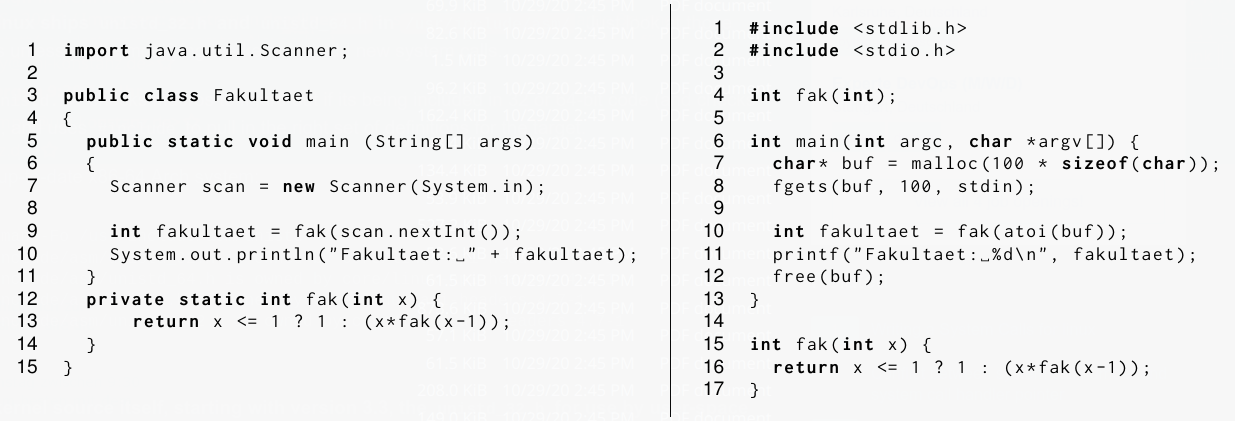
\includegraphics[keepaspectratio, width=\textwidth, height=\textheight-2\baselineskip-2\baselineskip]{img/300_c_vs_java.png} \\ \framebreak
 \end{center}

\end{frame}


 \begin{frame}[allowframebreaks]{Contents of the Programming Part}
    \begin{enumerate}
    \item C Language
        \begin{enumerate}
        \item Basics
        \item Pointers
        \item Dynamic Memory Management
        \item More on Types
        \item Inside Malloc
        \item Variables, Declarations \& Scope
        \item Large Program Organization
        \end{enumerate}
    \item UNIX
        \begin{enumerate}
            \item Arguments \& Environment
            \item Files \& IO
            \item Processes
            \item Inter-Process Communication
            \item Linking
        \end{enumerate}
    \end{enumerate}
 \end{frame}
 
 
\section{Compilers \& Linking}
\begin{frame}[allowframebreaks]{Compilers \& Linkers}
 \begin{center}
        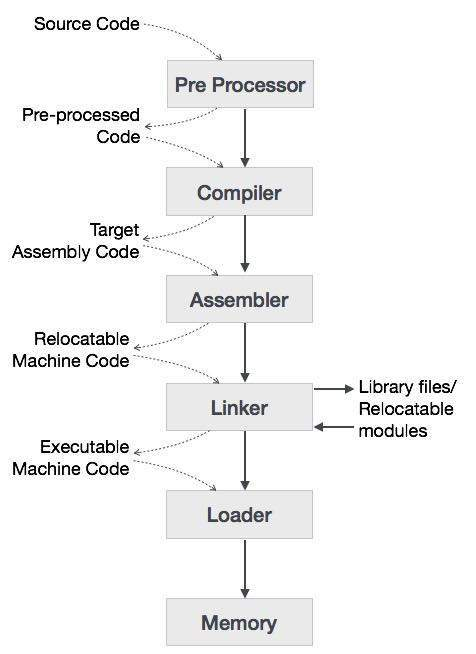
\includegraphics[keepaspectratio, width=\textwidth, height=\textheight-2\baselineskip-2\baselineskip]{img/210_compilation.jpg} \\ \framebreak
        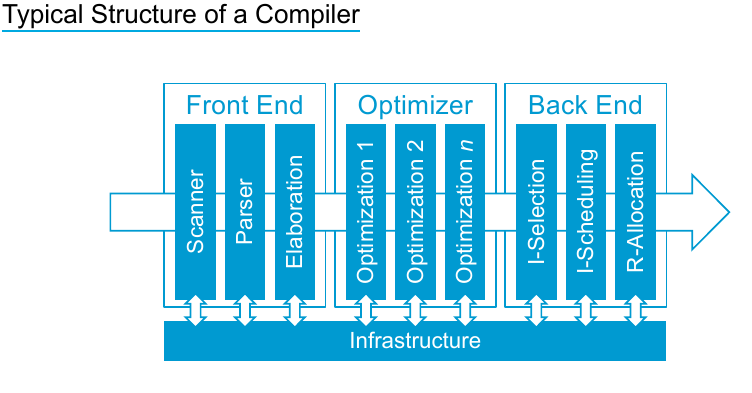
\includegraphics[keepaspectratio, width=\textwidth, height=\textheight-2\baselineskip-2\baselineskip]{img/200_compiler_architecture_overview.png} \\ \framebreak
      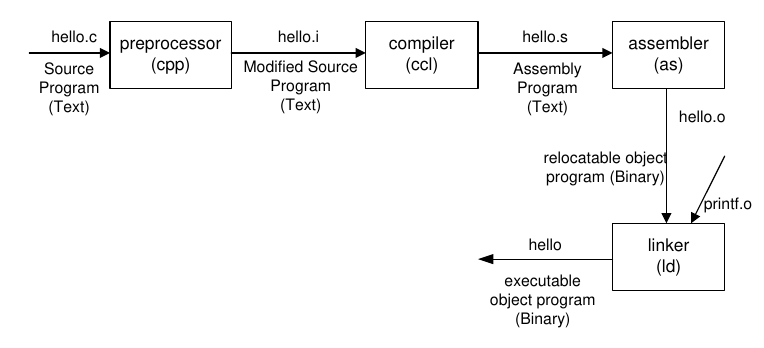
\includegraphics[keepaspectratio, width=\textwidth, height=\textheight-2\baselineskip-2\baselineskip]{img/211_compiler.png} \\ \framebreak
    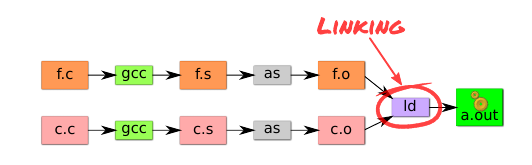
\includegraphics[keepaspectratio, width=\textwidth, height=\textheight-2\baselineskip-2\baselineskip]{img/220_linking_bigp.png} \\ \framebreak
    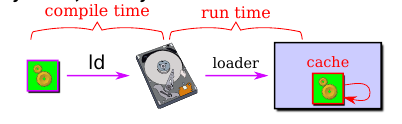
\includegraphics[keepaspectratio, width=\textwidth, height=\textheight-2\baselineskip-2\baselineskip]{img/212_compile_run.png} \\ \framebreak
    \includegraphics[keepaspectratio, width=\textwidth, height=\textheight-2\baselineskip-2\baselineskip]{img/221_linker_loader.png} \\ \framebreak
 \end{center}

\end{frame}


    
\section{References}
    \begin{frame}[allowframebreaks]
      \frametitle{References}
      \begin{tiny}
      \nocite{*}
      \printbibliography
      \end{tiny}
    \end{frame}


\end{document}
 
